% Created 2022-11-22 Tue 13:24
% Intended LaTeX compiler: pdflatex
\documentclass[a4paper,11pt]{article}
\usepackage[utf8]{inputenc}
\usepackage[T1]{fontenc}
\usepackage{graphicx}
\usepackage{longtable}
\usepackage{wrapfig}
\usepackage{rotating}
\usepackage[normalem]{ulem}
\usepackage{amsmath}
\usepackage{amssymb}
\usepackage{capt-of}
\usepackage{hyperref}
\usepackage[margin=1in]{geometry}
\usepackage{titlesec}
\usepackage{caption}
\usepackage{subcaption}
\usepackage{lipsum}
\author{Varghese Reji}
\date{}
\title{Classical and Quantum Optics\\\medskip
\large Assignment-2 Answers}
\hypersetup{
 pdfauthor={Varghese Reji},
 pdftitle={Classical and Quantum Optics},
 pdfkeywords={},
 pdfsubject={},
 pdfcreator={Emacs 28.2 (Org mode 9.5.5)}, 
 pdflang={English}}
\begin{document}

\maketitle

\section*{Problem 1}
\label{sec:orgcf1d1cb}
In the Einstein analysis we assume that the light radiation has a broad spectrum compared to the transition line. Let us now consider the contrary situation in which the spectral width of the light beam is much smaller than the linewidth of the transition. This is the kind of situation that occurs when a narrow-band laser beam interacts with as atom, inside a laser cavity or externally.
\begin{description}
\item[{(a)}] Explain why it is appropriate to write the spectral energy intensity of the beam as:
$$u(\omega') = u_\omega\delta(\omega'-\omega)$$
where \(\omega\) is the angular frequency of the beam, \(u_\omega\) is its energy density in \(Jm^{-3}\), and \(\delta(x)\) is the Dirac Delta function.
\item[{(b)}] Let us assume that the frequency dependence of the absorption probability follows the spectral lineshape function g\textsubscript{\(\omega\)}(\(\omega\)). This implies that the Einstein \(B\) coefficients will also vary with frequency. Explain why it is appropriate to write the frequency dependence of the Einstein \(B_{12}\) coefficient as:
$$B_{12} = \frac{g_2}{g_1} \frac{\pi^2c^3}{\hbar n^3\omega'^3} \frac{1}{\tau} g_{\omega}(\omega')$$
\item[{(c)}] Hence show that the total absorption rate defined as
$$W_{12} = N_1\int_{0}^{\infty} B_{12}(\omega') u(\omega')d\omega'$$
is given by:
$$W_{12} = N_1 \frac{g_2}{g_1} \frac{\pi^2c^3}{\hbar n^3\omega'^3} \frac{1}{\tau} u_{\omega}g_{\omega}(\omega')$$
\item[{(d)}] Repeat the arguement to show that the total stimulated-emission rate is given by:
$$W_{21} = N_2 \frac{\pi^2c^3}{\hbar n^3\omega'^3} \frac{1}{\tau} u_{\omega}g_{\omega}(\omega')$$
\end{description}
\subsection*{Solution}
\label{sec:org0fa8d77}
\begin{description}
\item[{(a)}] The formula of energy density is
\end{description}

\begin{equation}
\label{eq:org07ed0f1}
u(\omega) = \frac{\hbar \omega^3}{(c/n)^3 \pi^2}\frac{1}{\exp\left( \frac{\hbar \omega}{T k_B} \right) - 1}
\end{equation}

We are getting this by analysing the atomic transition. But in reality, there is a lot of other factors that affect the spectral width. Also, we are assuming that the light radiation had a broad spectrum compared to the transition line. But in this situation, we are taking the case which the 
spectral width of light beam is much smaller than line width of transition. That means, it is narrower than \ref{eq:org07ed0f1}. The best way to express this case is dirac delta function. So, it is appropriate to write the energy intensity as

$$u(\omega') = u_\omega\delta(\omega'-\omega)$$


\begin{description}
\item[{(b)}] We have the equations
\end{description}
\begin{equation}
A_{21} = \frac{\hbar \omega^3}{(c/n)^3 \pi^2}  B_{21}^{\omega}
\end{equation}

But \(A_{21}=\frac{1}{\tau}\). By solving this for \(B_{21}\),

\begin{equation}
B_{21}^{\omega} = \frac{A_{21}(c/n)^3 \pi^2}{\hbar \omega^3}
\end{equation}

\(B_{21}\) is the transition probability. But, the transition will depend on the frequency also. So, the total probability should be the product of probability for a particular frequency and \(B\). Then, the resultant \(B\) is,

\begin{equation}
\label{eq:orgfcf0a7f}
B_{21}^{\omega} = \frac{(c/n)^3 \pi^2}{\hbar \omega'^3\tau} g(\omega')
\end{equation}

By transforming this to \(B_{12}\),

\begin{equation}
B_{12}^{\omega} = \frac{g_2}{g_1}\frac{(c/n)^3 \pi^2}{\hbar \omega'^3\tau} g(\omega')
\end{equation}

\begin{description}
\item[{(c)}] We have the results, 

$$u(\omega') = u_\omega\delta(\omega'-\omega)$$
\end{description}
$$B_{12}^{\omega} = \frac{g_2}{g_1}\frac{(c/n)^3 \pi^2}{\hbar \omega'^3\tau} g(\omega')$$

The absorption rate is,

\begin{equation}
\label{eq:org470b655}
W_{12} = N_1\int_0^{\infty} B_{12}(\omega') u(\omega') d\omega'
\end{equation}
By substituting to this,

\begin{equation}
\begin{split}
W_{12} = &  N_1\int_0^{\infty} \frac{g_2}{g_1}\frac{(c/n)^3 \pi^2}{\hbar \omega'^3\tau} g(\omega')  u_\omega\delta(\omega'-\omega)d\omega'\\
= & N_1\frac{g_2}{g_1}\frac{(c/n)^3 \pi^2}{\hbar \omega^3\tau} g(\omega) u_\omega
\end{split}
\end{equation}

Then,

\begin{equation}
\label{eq:org1946559}
W_{12} =  N_1\frac{g_2}{g_1}\frac{(c/n)^3 \pi^2}{\hbar \omega^3\tau} g(\omega) u_\omega
\end{equation}

\begin{description}
\item[{(d)}] Applying \ref{eq:orgfcf0a7f} to \ref{eq:org470b655}, we will get,
\end{description}


\begin{equation}
\label{eq:orga549cd3}
W_{21} =  N_2 \frac{(c/n)^3 \pi^2}{\hbar \omega^3\tau} g(\omega) u_\omega
\end{equation}

\newpage
\section*{Problem 2}
\label{sec:org0e86cc0}
Consider an atom interacting with a monochromatic beam of light with angular frequency \(\omega\), where \(\omega\) is close to a transition frequency \(\omega\)\textsubscript{0}

\begin{description}
\item[{(a)}] Use the results of \hyperref[sec:orgcf1d1cb]{Problem 1} to show that the net rate of downward transitions (defined as the stimulated-emission rate less the absorption rate) is given by:
\end{description}


$$W_{21}^{net} = \frac{ c^3 \pi^2 }{h \tau n^3 \omega^2} \Delta N g_{\omega} u_{\omega}$$

where \(\Delta N = N_2 - \frac{g_2}{g_1} N_1\), \(u_\omega\) is the energy per unit volume of the beam, and \(g_\omega(\omega)\) is the spectral lineshape function.

\begin{description}
\item[{(b)}] Show that optical intensity is given by \(I=\frac{c u_\omega}{n}\)

\item[{(c)}] Consider a unit area of beam propagating in the \(+z\) direction through the medium. Show that the incremental increase in the intensity dI in a length element dz is given by:
$$dI = W_{21}^{net} \hbar\omega dz$$.
\item[{(d)}] Hence show that the gain coefficient is given by:

$$ \gamma(\omega) = \frac{\lambda^2}{4 n^2 \tau} \Delta N g_\omega(\omega) $$
\end{description}

\subsection*{Solutions}
\label{sec:org91bc14d}
\begin{itemize}
\item (a) By taking the difference of \ref{eq:org1946559} and \ref{eq:orga549cd3},
\end{itemize}
$$W_{21}^{net} = \left(N_2-\frac{g_2}{g_1}N_1\right) \frac{(c/n)^3 \pi^2}{\hbar \omega^3\tau} g(\omega) u_\omega $$

But, \(\Delta N = \left(N_2-\frac{g_2}{g_1}N_1\right)\).

Then,

$$W_{21}^{net} = \Delta N \frac{(c/n)^3 \pi^2}{\hbar \omega^3\tau} g(\omega) u_\omega $$

\begin{description}
\item[{(b)}] By the definition of intensity, it is the power transmitted through unit area in space. \(u_\omega\) is the energy density for a particular frequency \(\omega\) and \(c\) is the speed of light in free space. \(n\) is the refractive index of medium.
\end{description}

In a unit time, the light beam travels \(c\) meters. Energy density is the energy per unit volume.  Let we consider a light beam as a cylinder with unit cross sectional area. It contains radiation energy E\textsubscript{\(\omega\)}. Then, the energy density inside the cylinder will be \(u_\omega = E/h\) where \(h\) is the height of cylinder. But we know that a wavefront will travel \(\frac{c}{n}\) meters per second in a medium. So, in unit time, it traveled \(\frac{c}{n}\) distance. To get this, let us divide both numerator and denominator of expression for \(u_\omega\) by \(t\). Then in the numerator, it will be the intensity by definition. Denominator will become \(\frac{c}{n}\). 

\(I = \frac{E}{t}, \frac{c}{n}=\frac{h}{t}\).

Then, 

$$\frac{In}{c} = u_\omega$$.

\(\Rightarrow\),

$$I = \frac{c u_\omega}{n}$$.

\begin{description}
\item[{(c)}] From the equation of radiative transfer, we know that
\begin{equation}
\label{eq:org730d8c5}
 \frac{dI}{dz} = -(I \alpha)
 \end{equation}
where \(\alpha\) is the absorption coefficient.
But, transition probability per unit time for absorption is given by the formula \(B_{12}\bar{J}\) where
$$\bar{J} = \int_0^{\infty} J_\nu g_\omega(\omega) d\omega$$
Using these, the absorption coefficient in this case is given by
$$dVdt \hbar\omega_0 N_1 B_{12}/2{-1} \int d\Omega \int d\omega g_\omega(\omega) I_\nu$$
Then, the energy absorbed out of a beam in frequency range \(d\omega\) and solid angle d\(\Omega\) in time dt and volume dV is
$$dVdtd\Omega d\omega \hbar\omega N_1 B_{12} g_\omega(\omega) I $$
Now, there is no change in cross sectional area. So, we can take \(dV=dz\). By plugg in these to the above equation, we will get
$$\alpha = \frac{\hbar\omega}{4\pi} N_1 B_{12} g_\omega(\omega)$$
For stimulated emission, calculations are same. So, the net absorption coefficient will be,
$$\alpha = \frac{\hbar\omega}{4\pi}  g_\omega(\omega)(N_1 B_{12}-N_2B_{21})$$
So,
$$\frac{dI}{dz} =- \frac{\hbar\omega}{4\pi}  g_\omega(\omega)(N_1 B_{12}-N_2B_{21}) I$$
Let us make some rearrangements.
\begin{equation}
\begin{split}
\frac{dI}{dz} = & \frac{\hbar\omega}{4\pi}  g_\omega(\omega)(N_1 B_{12}-N_2B_{21}) I \\
= & \frac{\hbar\omega}{4\pi}  \left(N_2-\frac{g_2}{g_1}N_1\right)\frac{(c/n)^3 \pi^2}{\hbar \omega^3\tau} g(\omega) \frac{u_\omega c}{n} \\
= & W_{21}^{net} \hbar\omega
\end{split}
\end{equation}
\(\Rightarrow\)
$$dI =W_{21}^{net} \hbar\omega dz $$\footnote{Ref: Radiative Prosesses in Astrophysics, Lightman.}

\item[{(d)}] Gain coefficient \(\gamma\) is defined in the equation,

$$\frac{dI}{dz} = \gamma I$$
\end{description}

In previous questions, we got that,

$$\frac{dI}{dz} = W_{21}^{net} \hbar \omega $$

\(\Rightarrow\)

\begin{equation}
\begin{split}
\frac{dI}{dz} = & W_{21}^{net} \hbar \omega \\
= & \Delta N \frac{(c/n)^3 \pi^2}{\hbar \omega^3\tau} g(\omega) u_\omega \hbar \omega \\
= & \Delta N \frac{(c/n)^2 \pi^2}{\hbar \omega^3\tau} g(\omega) \frac{c u_\omega}{n} \hbar \omega\\ 
= & \Delta N \frac{(c/n)^2 \pi^2}{\hbar \omega^3\tau} g(\omega)  \hbar \omega I\\ 
= & \Delta N \frac{(c/n)^2}{4\nu^2\tau} g(\omega) I\\ 
= & \Delta N \frac{\lambda^2}{4n^2 \tau} g(\omega) I\\ 
\end{split}
\end{equation}

\(\Rightarrow\)

$$\gamma = \Delta N \frac{\lambda^2}{4n^2 \tau} g(\omega) I$$

\newpage
\section*{Problem 3}
\label{sec:org7a9a878}
Calculate the fraction of energy of a 00-mode laser beam with beam radius \(w\) within a distance \(w\) from the beam centre.
\subsection*{Solution}
\label{sec:org9db3b7d}
The electric field at a distance for 00-mode is given by

$$\mathcal{E}=\mathcal{E}_0\exp\left(-\frac{r^2}{w^2}\right)$$

Energy density of an electric field is given by, \(u=\frac{1}{2}\epsilon_0\mathcal{E}^2\). 

Then, total energy in a particular distance \(r\) is given by,

$$E(r) = \int_V udV = \pi \epsilon_0 \mathcal{E_0}^2\int_0^r e^{-\frac{2r'^2}{w^2}} r'dr' $$ 

$$=\pi\epsilon_0\frac{w^2\left(1-\exp\left( \frac{-2 r^2}{w^2}\right)\right)}{4}$$

So, the fraction of energy in distance \(w\)

$$\frac{E(w)}{E(\infty)} = 1-e^{-2}=0.864 = 86.4\%$$
\newpage
\section*{Problem 4}
\label{sec:org3c7d930}
A helium-neon laser consists of a laser tube of length 0.3m with mirrors bonded to the end of the tube. The output coupler has a reflectivity of \(99\%\). The laser operates on the 632.8 nm transition of neon (relativve atomic mass 20.18), which has an Einstein A coefficient of \(3.4\times 10^6s^{-1}\). The tube runs at \(200^oC\) and the laser transition is Doppler-broadened. On the assumption that the only loss in the cavity is through the output coupler, that the average refractive index is equal to unity, and that the laser operates at the line centre, calculate:
\begin{description}
\item[{(a)}] the gain coefficientt in the laser tube;
\item[{(b)}] the population inversion density.
\end{description}
\subsection*{Solution}
\label{sec:org0209914}
\(L=0.3m, R_2=0.99, \lambda = 632.8nm\), relative atomic mass = 20.18, A=3.4\texttimes{} 10\textsuperscript{6} s\textsuperscript{-1}, T=200\textsuperscript{oC}
\begin{description}
\item[{(a)}] Gain coefficient, $$\gamma=-\frac{1}{2L}\ln(R_1R_2)-\frac{1}{2L}\ln(k)$$
\end{description}
Then,
$$\gamma = 0.01675$$
\begin{description}
\item[{(b)}] Relation between gain coefficient \(\gamma\) and population inversion density \(\Delta N\) is given by the formula,
\end{description}

$$\gamma(\omega) 
  = \frac{\lambda^2}{4 \Delta N \tau n^2 g_{\omega}(\omega)}$$

where,

$$g_\omega(\omega) = \frac{c}{\omega_0} \sqrt{\frac{m}{2 T \pi k_B}} \exp\left( \frac{mc^2 (\omega - \omega_0)^2}{-2 T k_B \omega_0} \right)$$

But,

\(\omega\)\textsubscript{0} =  2.97724399494\texttimes{} 10\textsuperscript{15} Hz \(\approx\) 2.977 PHz


If we are evaluating at the line center, \(\omega=\omega_0\).

Then, \(g_\omega(\omega) \approx 9.136\times 10^{-11}\)

$$ \Delta N 
  = \frac{\lambda^2}{4 \gamma(\omega_0) \tau n^2 g_{\omega}(\omega_0)}$$

\(\tau = \frac{1}{A}, n=1\)

Then,

$$ \Delta N = \frac{A \lambda^2}{4\gamma(\omega_0) g_{\omega} (\omega_0)} = 222423.650574 $$
\newpage
\section*{Problem 5}
\label{sec:orge51c31f}
Estimate the Doppler and collision line widths of emission from \(H_2O\) molecules at \(\lambda = 0.5\mu m\), at 300K and atmospheric pressure. Assume the collision cross-section to be the same as the geometrical size of the molecule.

\subsection*{Solution}
\label{sec:org2b55bf3}
Given, \(\lambda = 0.5\mu m\), T=300K.

Let us consider the maximum possible geometrical area, which is in the plane perpendicular to \(z\) axis which pass through the oxygen atom. The angle between hydrogen atoms is \(104.45^o\), and length of one handle is \(l=95.84 pm\). \footnote{\url{https://en.wikipedia.org/wiki/Chemical\_bonding\_of\_water}}.And Atmospheric pressure is P=101325 Pa.

From Kinetic theory of gasses, we will get

\begin{equation}
\label{eq:orgd6d7994}
\tau_{col} \sim \frac{1}{\sigma P} \left(\frac{\pi m k_B T}{8}\right)^{\frac{1}{2}}
\end{equation}

m = 2m\textsubscript{H} + m\textsubscript{O} = 17m\textsubscript{H};
\(\sigma\) = \(\pi\) l\textsuperscript{2} \(\sin\)(104.45) = 2.70596603659\texttimes{} 10\textsuperscript{-20} m\textsuperscript{2} 

\(\therefore\)
$$\tau_{col} = 2.47784340277\times10^{-9}s$$

Then, linewdith, $$\Delta\omega_{col} = 2.53574753762\times10^9 s= 2.526 GHz$$

The linewidth by doppler broadening is given by the formula,

\begin{equation}
\label{eq:org222a7ef}
\Delta\omega_{Doppler} = \frac{4\pi}{\lambda} \left(\frac{2 k_B T  \ln 2}{m}\right)^{\frac{1}{2}} 
\end{equation}

Then, we will get,

$$\Delta\omega_{Doppler} = 1.13001722187\times 10^{10} = 11.30 GHz$$

\newpage
\section*{Problem 6}
\label{sec:org785bfd0}
Monochromatic light is scattered at \(90^o\) from a cell containing \(10^{-16}\) g particles in suspension at 300K. Estimate the coherence time and linewidth of the scattered light.
\subsection*{Solution}
\label{sec:org5b19e73}

The wavelength is not specified. So, assume that \(\lambda = 500nm\). T=300K
We can consider the scattering in this case like reflection from a moving mirror. The particles in this is in thermal motion. So, using kinetic theory, the kinetic energy of each particle in each direction is \(\frac{1}{2}k_BT\).

Here, the scattering is in \(90^o\). So, we can consider the line of sight along the path of reflected ray. We need to consider the motion of particle in that direction only. Let us take that direction as \(x\). Then, we can write,

$$\frac{1}{2} m v_x^2 = \frac{1}{2} k_B T$$.

Then, $$v_x = \sqrt{\frac{k_BT}{m}} = 2.034\times 10^{-1} m/s = 20.34cm/s$$

The Doppler shift can be written as

$$\frac{\delta\lambda}{\lambda} = \frac{v_x}{c} = 6.782\times10^{-10}$$

Then, 

$$\delta\lambda = \frac{v_x\lambda}{c} = 3.3911\times 10^{-16} m = 3.391\times 10^{-7}nm $$

The coherence time is given by the formula

$$\tau_c = \frac{\lambda^2}{c\delta \lambda} = \frac{\lambda}{v_x}$$

Then,

$$\tau_c = 1.667\times 10^{-15} = 1.667 fs $$

\newpage
\section*{Problem 7}
\label{sec:org0023f6f}
Several output modes of a laser, indicated by the small integer m which lies between, say, +5 and –5, are represented by the waves 
\begin{equation}
E_n=a\exp\left[-i[(\omega_0+n\omega_1)t+\phi_n]\right]
\end{equation}
where \(\omega_1\) is the mode-spacing frequency. To illustrate mode-locking, calculate the wave resulting from superposition of these modes when (a) \(\phi_n\) is a random variable and (b) all \(\phi_n = 0\). (It is convenient to do this by computer.) 
\subsection*{Solution}
\label{sec:orgb90a08b}
The solution of this is done in python. You can see the code \href{https://github.com/varghesereji/Coursework\_assignments/blob/main/CQO/Ass\_2/Problem\_7\_answer\_code.py}{here.}
\begin{description}
\item[{(a)}] In this case, values of \(\phi\) is random.  The mode-locked pulses will be as shown in the figure below.
\end{description}
\begin{center}
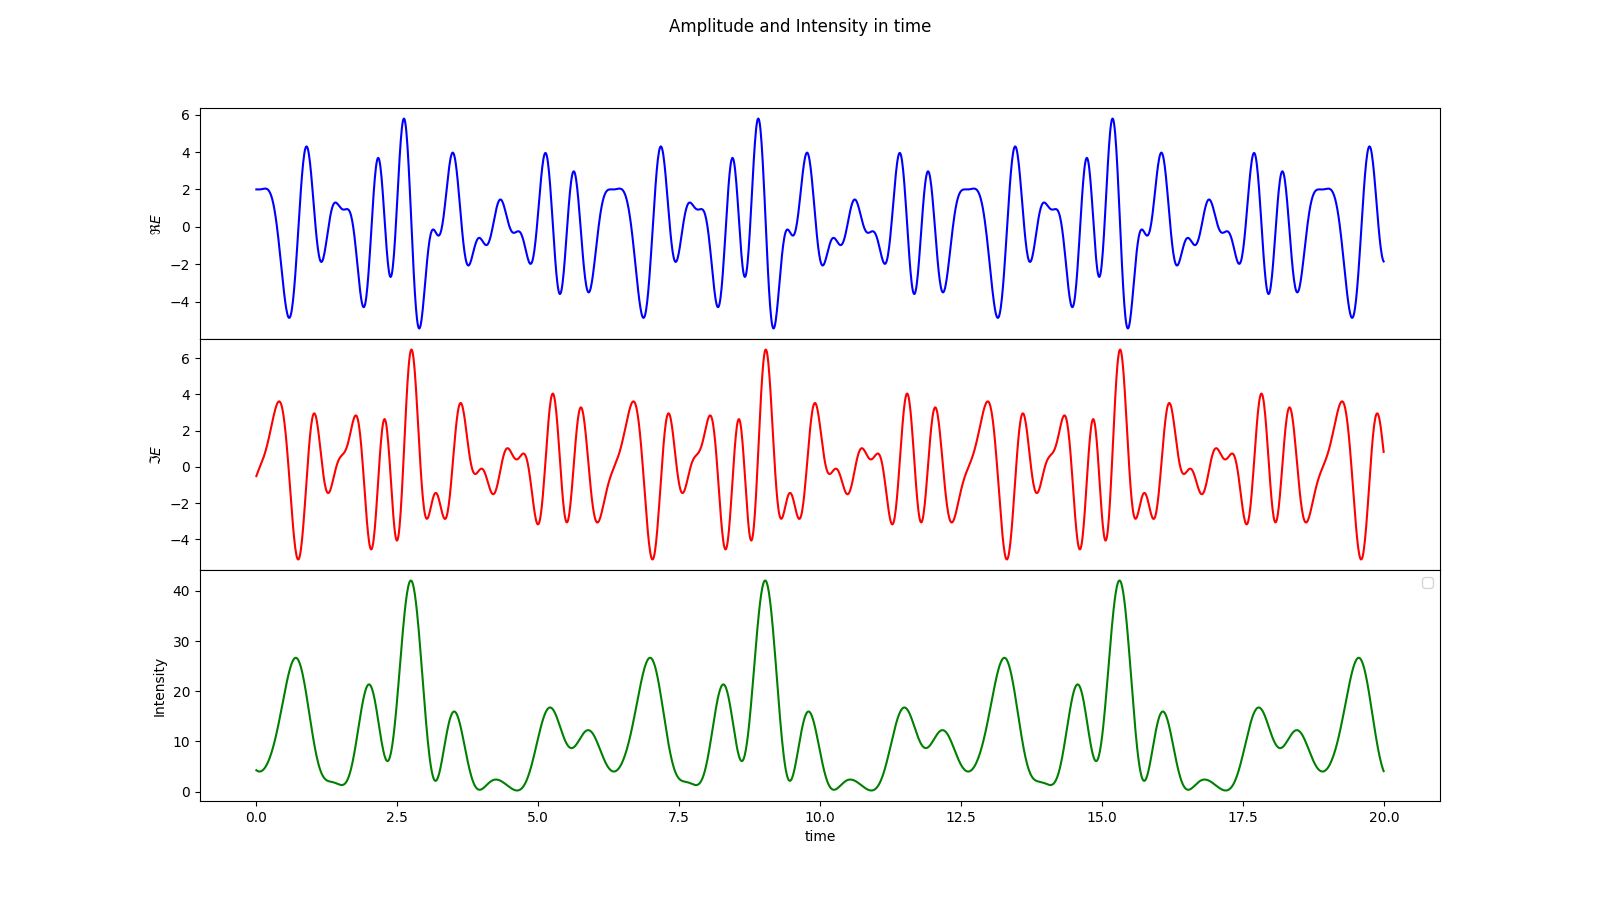
\includegraphics[width=.9\linewidth]{pr_7_a.png}
\end{center}
\begin{description}
\item[{(b)}] Here, \(\phi\) is 0. The pulses is shown in the figure below.
\end{description}
\begin{center}
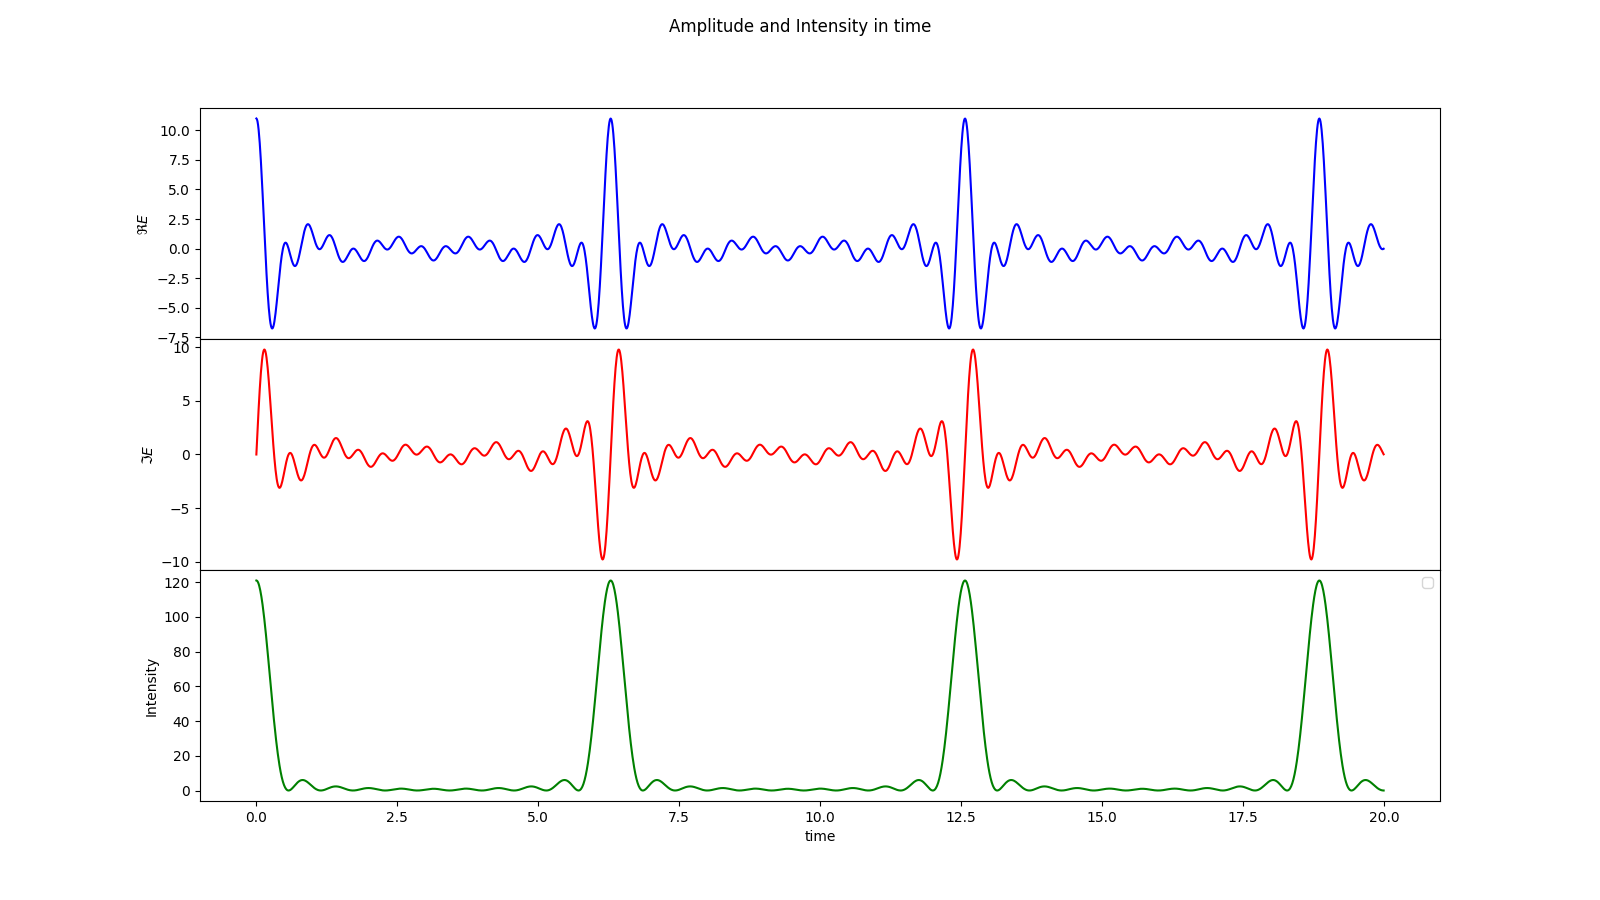
\includegraphics[width=.9\linewidth]{pr_7_b.png}
\end{center}

\newpage

\section*{Problem 8}
\label{sec:org913ffb8}
Calculate and plot the intensity profile across the diameter of a laser spot of the \(TEM_{00}\) and \(TEM_{10}\) modes emanating from a resonator with circular symmetry. Next, do the same for a resonator with rectangular symmetry. Here, plot along the X axis. You may assume any numerical values of geometric parameter for the resonators if needed.

\subsection*{Solution}
\label{sec:org6446ed4}

For cylindrical cavity, the beam is Laguerre-Gaussian beam. It is given by the equation, (There is angle dependence actually. But we are looking only on intensity. Then, terms with angle will go. So, I am not adding it here. Also, take \(w=1\))

$$\mathcal{E}_{mn}^L(r) = r^n L_{mn}(2r^2)\exp(-r^2)$$ \footnote{Ref: \url{https://laser.physics.sunysb.edu/\_alex/tmodes/webreport.html}}

where,

$$L_{mn}(r) = \frac{e^r r^{-n}}{m!}\frac{d^m}{dr^m}\left(e^{-r} r^{n+m}\right)$$

For m=0, n=0, L\textsubscript{mn}(r)=1 Then, the plot is simply gaussian.

$$\mathcal{E}_{00} = e^{-r^2}$$

For m=1, n=0,

$$L_{10} =  \left( 1-r \right)$$ \footnote{Ref: Griffiths, Quantum Mechanics.}



Then,

$$\mathcal{E}_{10} = \left( 1-r  \right) e^{-r^2}$$


The amplitude for a particular mode in rectangular cavity is given by
$$\mathcal{E}_{mn}(x,y) = \mathcal{E}_0H_m\left(\frac{\sqrt{2} x}{w}\right)H_n\left(\frac{\sqrt{2} y}{w}\right)e^{-\frac{x^2+y^2}{w^2}}$$

\(H_m\) and \(H_n\) are Hermite polynomials.

For simplicity, take \(\mathcal{E}_0 = 1, w=1\). Then,

$$\mathcal{E}_{mn}(x,y) = H_m\left(\sqrt{2} x\right)H_n\left(\sqrt{2} y\right)e^{-(x^2+y^2)}$$

$$\mathcal{E}_{00}(x,y) = e^{-(x^2+y^2)}$$
$$\mathcal{E}_{10}(x,y) = 2x e^{-(x^2+y^2)}$$
The figure had been shown below.

\begin{center}
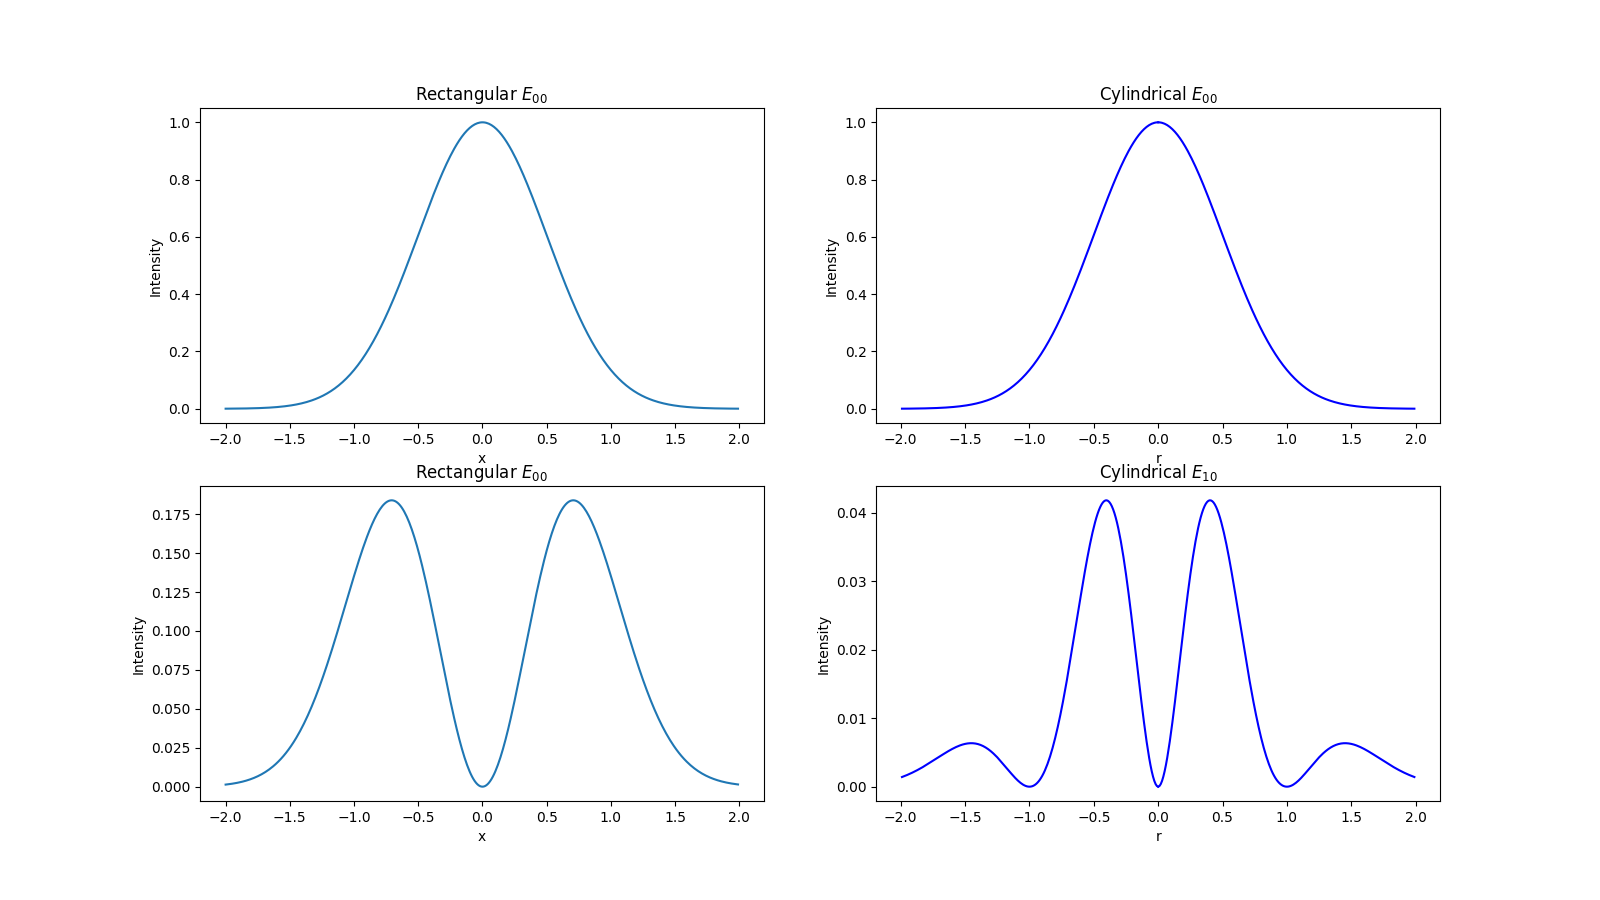
\includegraphics[width=.9\linewidth]{laser_intensity.png}
\end{center}

\newpage
\section*{Problem 9}
\label{sec:orgd8c1546}
A material has six energy levels A to F at 2, 1.9, 1.7, 1.6, 1.1 and 0.4 eV above the ground state, G. The time constants for the various possible transitions in nanoseconds are shown in figure (Not adding here.) Suggest possible lasers working with this material, and give the pump and output wavelendths of each one.
\subsection*{Solution}
\label{sec:org35f67cb}

For a laser, we have to satisfy condition to happen the lasing.
\begin{description}
\item[{(a)}] The lowest level is the ground state
\item[{(b)}] Uppermose state must be connected to the ground state by a short time constant if optical pumping is to be used.
\item[{(c)}] One pair of levels, which will be lasing levels must be connected weakly, i.e. the time constant for transitions between them must be long compared to the others involved
\item[{(d)}] The upper laser level must not have a faster competing transition to another level, excluting the ground state of optical pumping is used.
\end{description}

\subsubsection*{Energy levels}
\label{sec:org476d636}
\begin{center}
\begin{tabular}{|c|c|c|c|c|c|c|c|}
\hline
Level & A & B & C & D & E & F & G\\
\hline
Energy from G(eV) & 2 & 1.9 & 1.7 & 1.6 & 1.1 & 0.4 & 0\\
\hline
\end{tabular}
\end{center}

\subsubsection*{Time constants between different levels in nanoseconds.}
\label{sec:org45662f4}
\begin{center}
\begin{tabular}{|c|c|c|c|c|c|c|}
\hline
B & 0 & - & 50 & 50 & 10\textsuperscript{4} & 0\\
\hline
C & 10 & 50 & - & 10\textsuperscript{4} & 10\textsuperscript{4} & 0\\
\hline
D & 0 & 50 & 10\textsuperscript{4} & - & 0 & 10\textsuperscript{4}\\
\hline
E & 0 & 10\textsuperscript{4} & 10\textsuperscript{4} & 0 & - & 100\\
\hline
F & 0 & 0 & 0 & 10\textsuperscript{4} & 100 & -\\
\hline
G & 10 & 10 & 0 & 0 & 10\textsuperscript{4} & 10\\
\hline
 & A & B & C & D & E & F\\
\hline
\end{tabular}
\end{center}

The lasing will happen when the time constants are sufficiently high. So, we need to look only for such cases from the above table. This condition had been satisfied in 5 cases with time constant \(10^{5} ns\). Those are,  C\(\rightarrow\) D, B\(\rightarrow\) E, C\(\rightarrow\) E, C\(\Rightarrow\) F and E\(\rightarrow\) G.

\subsubsection*{Levels for lasing}
\label{sec:orgb96d50c}

\begin{center}
\begin{tabular}{llrrrrl}
\hline
Higher & Lower & Em\textsubscript{2} & Em\textsubscript{1} & Em\textsubscript{2}-Em\textsubscript{1} & \(\lambda\) & Comment\\
 &  & (eV) & (eV) & (eV) & (\(\mu\) m) & \\
\hline
C & D & 1.7 & 1.6 & 0.1 & 12.42375 & 4L\\
C & F & 1.7 & 0.4 & 1.3 & 0.95567308 & 4L\\
C & E & 1.7 & 1.1 & 0.6 & 2.070625 & 4L\\
B & E & 1.9 & 1.1 & 0.8 & 1.5529688 & 3L\\
E & G & 1.1 & 0 & 1.1 & 1.1294318 & 3L\\
\hline
\end{tabular}
\end{center}


To reach this higher metastable state, pumping level should be larger than that. Now, let us look on the required pumping levels and pumping energy. The time constant for this should be low.

\subsubsection*{Pumping wavelengths}
\label{sec:org02895f2}
\begin{center}
\begin{tabular}{lllrrrrl}
\hline
Upper & Higher & Lower & E\textsubscript{2} & E\textsubscript{1} & E\textsubscript{2}-E\textsubscript{1} & \(\lambda\) & Comment\\
Metastable & Pumping & Pumping & (eV) & (eV) & (eV) & (micron) & \\
State & level & level &  &  &  &  & \\
\hline
C & A & G & 2 & 0 & 2 & 0.6211875 & 4L\\
C & B & G & 1.9 & 0 & 1.9 & 0.65388158 & 4L\\
B & B & G & 1.9 & 0 & 1.9 & 0.65388158 & 3L\\
B & B & C & 1.9 & 1.7 & 0.2 & 6.211875 & 3L\\
B & B & D & 1.9 & 1.6 & 0.3 & 6.211875 & 3L\\
E & E & F & 1.1 & 0.4 & 0.7 & 1.7748214 & 3L\\
\hline
\end{tabular}
\end{center}

\subsubsection*{Possible Lasing Actions}
\label{sec:org3efddd7}

The output wavelength should be larger than pump wavelength. So, we will filter out other cases.

\begin{center}
\begin{tabular}{|c|c|c|c|c|c|c|c|c|}
\hline
E\textsubscript{1} & E\textsubscript{2} & Em\textsubscript{2} & Em\textsubscript{1} & \(\tau\) & \(\tau\) & Output & pump & Comment\\
 &  &  &  & pumping & lasing & \(\lambda\) & \(\lambda\) & \\
 &  &  &  & (ns) & (ns) & (\(\mu\) m) & (\(\mu\) m) & \\
\hline
G & A & C & D & 10 & 10000 & 12.42375 & 0.6211875 & 4L\\
G & B & C & D & 10 & 10000 & 12.42375 & 0.65388158 & 4L\\
G & A & C & F & 10 & 10000 & 0.95567308 & 0.6211875 & 4L\\
G & B & C & F & 10 & 10000 & 0.95567308 & 0.65388158 & 4L\\
G & A & C & E & 10 & 10000 & 2.070625 & 0.6211875 & 4L\\
G & B & C & E & 10 & 10000 & 2.070625 & 0.65388158 & 4L\\
G & B & B & E & 10 & 10000 & 1.5529688 & 0.65388158 & 3L\\
\hline
\end{tabular}
\end{center}
\end{document}